%File: formatting-instruction.tex
\documentclass[letterpaper]{article}
\usepackage{aaai}
\usepackage{times}
\usepackage{helvet}
\usepackage{courier}
\usepackage{graphicx}
\usepackage{algorithm}
\usepackage[noend]{algorithmic} 
%\usepackage{cite }
%\usepackage{natbib}
\frenchspacing
\setlength{\pdfpagewidth}{8.5in}
\setlength{\pdfpageheight}{11in}
\pdfinfo{
/Title (Streaming Fact Extraction for Wikipedia Entities at Web-Scale)
/Author (Morteza Shahriari Nia, Christan Grant, Yang Peng, Daisy Zhe Wang, Milenko Petrovic)}
\setcounter{secnumdepth}{0}  
 \begin{document}
% The file aaai.sty is the style file for AAAI Press 
% proceedings, working notes, and technical reports.
%
\title{Streaming Fact Extraction for Wikipedia Entities at Web-Scale}
\author{Morteza Shahriari Nia$^*$, Christan Grant$^*$, \\
\bf \large Yang Peng\thanks{All authors contributed equally.}, Daisy Zhe Wang\\
Data Science Research Lab\\
University of Florida\\\
Gainesville, Florida 32611\\
\And Milenko Petrovic\\
Institute for Human and Machine Cognition\\ 15 SE Osceola Ave \\\ Ocala, Florida 34471
}



\maketitle
\begin{abstract}
\begin{quote}
Wikipedia.org is the largest online resource for free information and is maintained by a small number of volunteer editors.
The site contains 4.3 million english articles; these pages can easily be neglected, becoming out of date.
Any news-worthy event may require an update of several pages.
To address this issue of stale articles we create a system that reads
in a stream diverse web documents and recommends
facts to be added to specified Wikipedia pages.
We developed a three-stage streaming system that creates models of Wikipedia pages,
filters out irrelevant documents and 
extracts facts that are relevant to Wikipedia pages.
The systems is evaluated over a 500M page web corpus and 139 Wikipedia pages.
Our results show a promising framework for fast fact extraction from arbitrary web pages for Wikipedia.

\end{quote}
\end{abstract}

\noindent 

Wikipedia.org (WP) is the largest and most popular general reference work on the Internet.
The website is estimated to have nearly 365 million readers worldwide.
An important part of keeping WP usable it to include new and current content.
%An important challenge in maintaining WP, the most popular web-based, collaborative, multilingual KB on the internet, is making sure its contents are up-to-date.
Presently, there is considerable time lag between the publication of an event and its citation in WP\@.
The median time lag for a sample of about 60K web pages cited by
 WP articles in the \textit{living\_people} category is over a year
 and the distribution has a long and heavy tail
 \cite{frank2013building}.
%Also, the majority of WP entities have updates on their associated article much less frequently than their mention frequency.
Such stale entries are the norm in any large reference work because the number
of humans maintaining the reference is far fewer than the number of entities.

Reducing latency keeps WP relevant and helpful to its users.
Given an entity page, such as \textsl{wiki/Boris\_Berezovsky\_(businessman)}\footnote{http://en.wikipedia.org/wiki/Boris\_Berezovsky\_(businessman)},
possible citations may come from a variety of sources.
Notable news may be derived from newspapers, tweets, blogs and a variety of
different sources include Twitter, Facebook, Blogs, arxiv, etc.
However, the actual citable information is a small percentage of the total documents that appear on the web.
%We develop a system to read streaming data and filter out articles that are candidates for citations. 
%The goal of this system is to read web documents and recommend citable facts (attributes) for WP pages.
To help WP editors, a system is needed to parse through terabytes of documents 
and select facts that can be recommended to particular WP pages.


Previous approaches are able to find relevant documents given a list of WP
entities as query nodes \cite{mcnamee2012hltcoe}
 \cite{dalton2013bi}\,
\cite{Bonnefoy:2013:WDE:2484028.2484180, Balog:2013:CCR:2484028.2484151,ji2011knowledge}.
Entities of three categories \textit{person}, \textit{organization} and \textit{facility} are considered.
This work involves processing large sets of information to determine which facts may contain references to a WP entity. 
This problem becomes increasingly more difficult when we look to extract relevant facts from
each document.
Each relevant document must now be parsed and processed to determine if a sentence or paragraph is worth being cited.
% Reorder this paragraph
%The challenges that we address are: first finding documents that contain useful information about the entity (avoid spams, documents that do not have direct information about the entity even though they mention them, etc), the scale where \textit{stream processing} nature of the system makes it suitable to avoid batch processing natures of Hadoop and operate in the realm of streams such as twitter storm~\footnote{http://storm-project.net/} which similarly processes unblounded streams of twitter data or Spark Streaming~\footnote{http://spark.incubator.apache.org/}. Further, this is called streaming because data is being generated as time goes
%on and for each extraction we should only consider current or past data. As other Natural Language Processing tasks, precision and recall of the extent we can extract slot values are very important metrics that we will discuss later on. Having to balance between infamous and obscure entities, dealing with slots that can be very broad (e.g.\ things that an entity is affiliated with) or very specific (such as cause of death of a \textit{person} entity).

Discovering facts across the Internet that are relevant and citable to the WP entities is a non-trivial task.
%For example, a take a sentence from the Internet:
Here we produce an example sentence from a webpage: 

%\texttt{Boris Berezovsky made his fortune in Russia in the 1990s when the
%country went through privatisation of state property and `robber capitalism', and passed away March 2013.}
``{\small \texttt{Boris Berezovsky, who made his fortune in Russia in the 1990s, passed away March 2013.}}''

After parsing the sentence, we must first note that there are two entities named \textit{Boris Berezovsky} WP; one a businessman and the other a pianist.
Any extraction needs to take this into account and employ a viable distinguishing policy (entity resolution).
Then, we match the sentence to find a topic such as \textit{DateOfDeath} valued at \textit{March 2013}.
Each of these operations is expensive so an efficient framework is necessary to execute these operations at web scale.
%Other examples that this system can answer could be `Who a person has met during a certain period of time?', `Who are the employees of this organization?', `Who has met who in this facility at a certain time?'.


In this paper, we introduce an efficient fact extraction system or given WP entities from a time-ordered document stream.
Fact extraction is defined as follows: match each sentence to the generic sentence structure of \{\textit{subject} --- \textit{verb} --- \textit{adverbial/complement}\}~\cite{sentencePatterns08}.
The first \textit{subject} represents the entity (WP entity) and \textit{verb} is the relation type (slot) we are interested in (e.g. Table~\ref{table:slotNameOntology}).
The third component, \textit{adverbial/complement}, represents the value of the associated slot.
In our example sentence, the entity of the sentence is \textit{Boris Berezovsky} and the slot we extract is
\textit{DateOfDeath} with a slot value of \textit{March 2013}.
The resulting extraction containing an entity, slot name and slot value is a \emph{fact}.


%Slot extraction is a challenging task in current state of the art Knowledge Bases (KB).
%Popular graphical KB such as Freebase or DBPedia keep data in structured format where entities
%are connected via relationships (slots) and the associated attributes
%(slot values).
%Our system can be used as an aid to recommend factual updates to such KBs.


Our system contains three main components.
First, we pre-process the data and build models representing the WP query entities.
Next, we use the models to filter a large stream of documents so they only contain candidate citations.
Lastly, we processes sentences from candidate extractions and return slot values. 
% EITHER SAY WHAT IT MEANS OR GIVE EXAMPLES OR COMMENT IT
%We build a modular system that allows us to explore the nuances of the training data and queries. 
Overall, we contribute the following:
\begin{itemize} %[noitemsep,nolistsep]
\item Introduce a method to build models of WP name variations;% (Section~\ref{sec:entitymodel});
\item Built a system to filter a large amount of diverse documents using a natural language processing rule-based extraction system;% (Section~\ref{sec:slotfilling});
\item Extract, infer and filter entity-slot-value triples of information to be added to KB.%(Section~\ref{sec:constraintsandinference}).
\end{itemize}

\begin{table}
\caption{The set of possible slot name for each entity type.}
\centering
\label{table:slotNameOntology}

\setlength{\tabcolsep}{1pt}

\begin{tabular}{|c|c|c|}
\hline 
\textbf{{\small Person}} & \textbf{{\small Facility}} & \textbf{{\small Organization}} \\ 
\hline 
\begin{tabular}{@{}l@{}}{\small Affiliate }\\ {\small AssociateOf }\\  {\small Contact\_Meet\_PlaceTime} \\ {\small AwardsWon }\\ 
{\small DateOfDeath }\\ 
{\small Titles}\\
{\small FounderOf}\\
{\small EmployeeOf}\end{tabular}
  &
   \begin{tabular}[b]{l}{\small Affiliate }\\ {\small Contact\_Meet\_Entity} \end{tabular} 
   & 
   \begin{tabular}{@{}l@{}}{\small Affiliate }\\ {\small TopMembers} \\ {\small FoundedBy}\end{tabular} \\ 
\hline 
\end{tabular} 
\end{table}

\section{System}

In this section, we introduce the main components of the system.
Our system is built with a pipeline style architecture giving it the advantage to run each section separately to allow stream processing without blocking the data flow of components (Figure~\ref{fig:system}).
The three logical components are divided into sections entitled \textit{Model} for entity resolution purposes,
\textit{Wikipedia Citation} to annotate cite-worthy documents,
and \textit{Slot Filling} to generate the actual slot values.


To discover facts for a single WP entity, the first step is to extract aliases of the entity.
%We use several approaches to get as many viable aliases as possible.
We extract several name variations from the Wikipedia.org API and from the WP entity page.
Also, if the entity type is \textit{person} we can change the order of user names to increase coverage (e.g. `Boris Berezovsky' $\rightarrow$ `Berezovsky, Boris').
Next, we iterate over documents in the stream and filter out all documents that do not explicitly contain a string matching 
the list of entities.
To extract relevant facts we perform pattern matching over each sentence that matches the entity based on a dictionary
of patterns.
If a sentence activates one of the patterns in the dictionary we emit this sentence as a candidate contribution
for the WP entity.
With the candidate set, we infer new facts from the set and clean up the set
by removing the set of values that violate a list of constraints such as duplicates.
%Lastly, we try to infer a new set of facts based on a list of rules.

%As a match is found from the content of the sentence to the patterns that we have generated regarding slot name, the associated slot value is extracted as a final result.

%\ceg{Discuss current system first. If you want to keep the decisions points that led to the current architecture, make it a subsection.}

\begin{figure}
%\hspace{-10mm}
  \centering
%  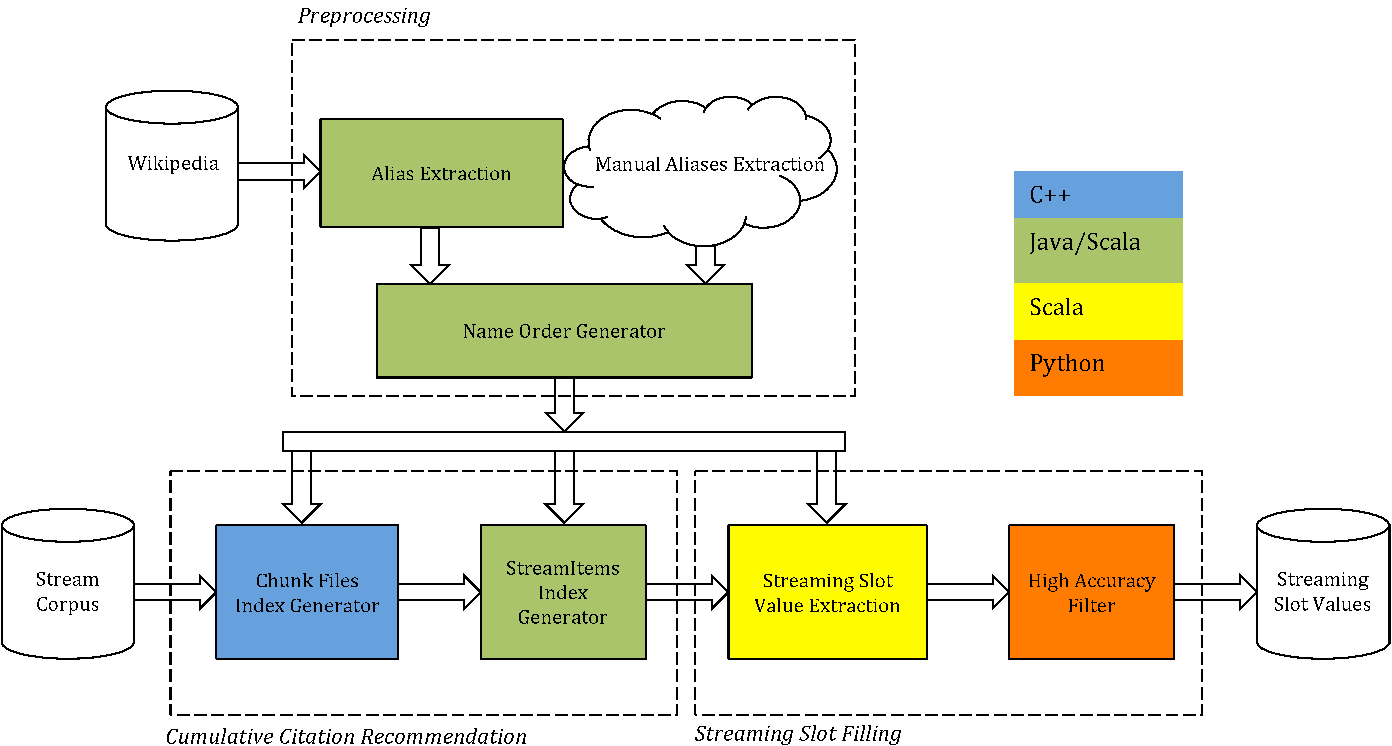
\includegraphics[width=6in]{./images/sdl-eps-converted-to.pdf}
  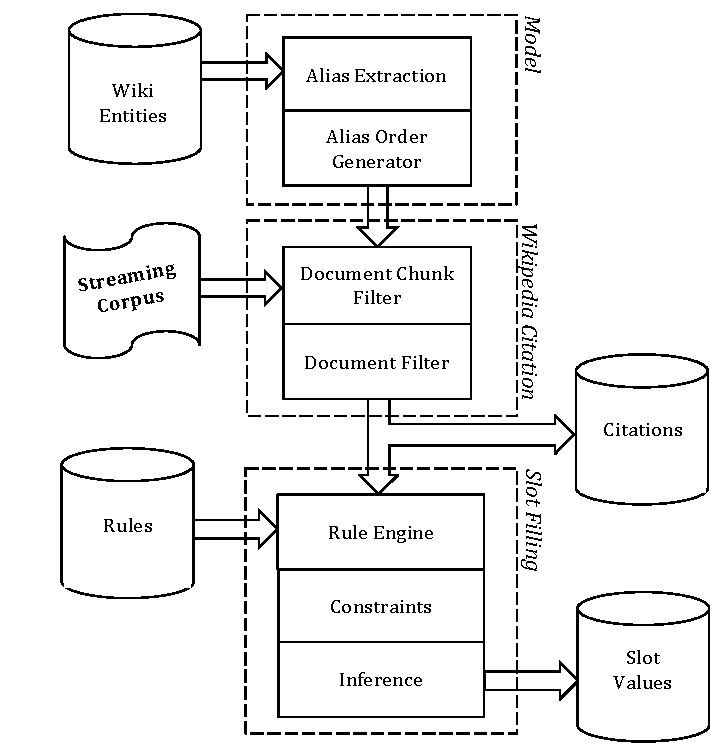
\includegraphics[width=8.5cm]{./images/System_Diagram_with_model_Vertical-crop.pdf}
% http://convert.neevia.com/pdfconvert/
  %\vspace*{-.1in} 
  \caption{System Architecture.
  Components are logical groups noted with dotted boxes.}
  \label{fig:system}
  %\vspace*{-.2in}
\end{figure}



\subsection{Entity Model}
\label{sec:entitymodel}

We use the Wikipedia.org API to retrieve aliases. 
The API allows us to requests pages that redirect users to an entity page.
For example, if a WP user tries to access the \textsl{William Henry Gates} entry they are sent to the page for 
\textsl{Bill Gates} --- we treat  such redirects as aliases. 
To extract more aliases we parse the HTML source of a WP entity page.
Using regular expressions we extract the bold phrases of the initial paragraph as aliases.
This method provides several inline aliases from the wiki page.
In WP page for the businesman `Boris Berezovski' , there is a mention of `Boris Abramovich Berezovsky' given in bold in the wiki page which obtained by regular expression extraction.

%\ceg{Do we know how many additional aliases this method provides?}.
%\ceg{Do you want to give a more concrete example of how this might now work? It may be TMI.}
%As an example of when this might not wirk, is that there might be occasions that some other topic is written in bold typesetting in the first paraph apart from the entity aliases itself but these are very rare.

We pass the full set of \textit{person} entities through rules for generating alternate name orders.
This module produces various forms of expressing entity names and titles.
For example, \textsl{Bill Gates} can be written as \textsl{Gates, Bill}.
This allows the system to capture various notation forms of aliases that appear in text documents.
%We refer to this part as \textit{Alias Order Generator}.

\subsection{Wikipedia Citation}
The goal of this section is to use the models created to discover a set of documents that are relevant to the WP entity.
%We perform exact string matching and treat all the documents that mention an entity equally likely to be citable.
As a stream of documents come in we first perform a string match between the model aliases and document text. 
We use this technique as a first filter with confidence because previous work states non-mentioning
documents have a low chance of being citable in Wikipedia \cite{frank2013building}.
Given our large number of aliases we can be confident that if an alias does not appear in a document it does not need to be cited.

Our system streams in documents in the form of chunk files.
Each chunk file contains thousands of documents.
This corpus of documents is processed by a two-layer filter system referred to as \textit{Document Chunk Filter} and \textit{Document Filter}.
The purpose of these filters is to reduce I/O cost while generating slot values for various entities.
Document Chunk Filter removes the chunk files that do not contain a mention of any of the desired entities.
Each chunk file may contain thousands of documents --- each document is expensive to process.
The Document Filter removes documents that do not contain a mention of an entity.
This two-level filter allows us to perform detailed slower processing over a smaller set of documents.
Not all chunk files contain mention of the entities so filtering out large chunk files early saves on I/O and processing.
Document Chunk Filter discards non-mentioning chunk files and promotes chunk files as soon as an entity mention is found.
%Processing StreamItems on the other hand is done in Java with ideas in mind for later on extensibility by adding other Java libraries.
The document filter additionally notes the sentences that contain entity mentions.
This data is passed to the Slot Filling system.


% Note: Describe the algorithms of each phase
% Talk in abstract terms not implementation.
% Use formal representations (Math, SQL etc)


%\ceg{This section should be structured as follows:
%1: Introduce CCR (Motivation, Expectations)
%2: Our high level approach
%3: Discussion of our design (Like already discussed)
%}


\subsection{Slot Filling}
\label{sec:slotfilling}
%\ceg{See the previous note.}
Streaming Slot Filling (SSF) extracts fact values from sentences according to a list of patterns.
Table~\ref{table:slotNameOntology} lists the slot relationships that we looks to extract.
In Figure~\ref{fig:system} we refer to this task as \textit{Slot Filling}. 

%Slot filling is done by pattern matching documents with manually produced patterns for slots of interest.
%The way we do this is by observing a sentence that has a mention of the entity or one of its coreference.
%An anchor word in the sentence related to the slot name is located and we match either left or right of
%the anchor word for potential slot values. 



%In the data set, we are given a date range of documents as training data. Instead of building a classifier we use pattern matching methods to find corresponding slot values for entities. 
%Pattern matching is simple to manipulate results and implement. Additionally, a classifier approach is more difficult to evaluate and explain results due to the lack of proper training data.

SSF reads documents filtered by the Wikipedia Citation step and fetches and tags sentences containing WP entities.
All entities are extracted from the document using a natural language processing
tool\footnote{Lingpipe (available in the dataset) provides entity tags
and in-document coreference. http://alias-i.com/lingpipe/}.
In the next section, we describe how WP entities are matched against the set of patterns.
Following, we discuss our approach to inference over the extracted facts.

\begin{algorithm}
  \caption{Slot Value Extraction Pseudocode}
  \textbf{List of entities $\mathcal{E} = \{e_0, \ldots, e_{170}\}$}\\
  \textbf{List of patterns $P = \{p_0, \ldots, p_{|P|}\}$}\\
  \textbf{List of documents containing entities $\mathcal{S} = \{s_0, \ldots, s_{|\mathcal{S}|}\}$}\\

  \begin{algorithmic}%[1]
    \FOR{$si \in \mathcal{S}$}
    \FOR{$sentence \in si$}
    \FOR{$entity \in \mathcal{E}$}
    \IF{Contains($sentence$, $entity$)}
    \FOR{$pattern \in P $ suitable for $entity$} 
    \IF{Satisfies($sentence$, $pattern$)}
    \STATE Emit($sentence$, $pattern$)
  \ENDIF
\ENDFOR
          \ENDIF
        \ENDFOR
      \ENDFOR
    \ENDFOR
  \end{algorithmic}
\end{algorithm}


\subsubsection{Rule Engine}

%\textbf{Format of Patterns.}
A pattern is a template of a fact to be extracted and added to a WP entity.
Patterns are used to find and extract facts from text.
A pattern $\mathcal{P}$ is represented as a five-tuple $\mathcal{P} = \langle p_1, p_2, p_3, p_4, p_5 \rangle$.


The first value, $p_1$ represents the type of entity.
These entity types are in the set
 $ \{ \texttt{FAC}, \texttt{ORG}, \texttt{PER} \}$ 
where \texttt{FAC} represents a type of facility, \texttt{ORG} represents an organization and \texttt{PER} represents a person.
%\texttt{FAC}, \texttt{ORG} and \texttt{PER} are Lingpipe entity types.
 $p_2$ represents a slot name.
A list of slot names is present in Table~\ref{table:slotNameOntology}.
The third element $p_3$ is the pattern content --- 
a string found in the sentence that identifies a slot name.
The extractor looks specifically for pattern content.
The pattern evaluator uses a direction (\texttt{left} or \texttt{right}) found in $p_4$ to explore sentence.
The final element $p_5$ represents the slot value of a pattern. 
%When we match one pattern, we match all the 
%fields except the third field, which is extracted as the final result.
The type of slot value may be the entity type labeled by the named entity extractor,
a noun phrase (\texttt{NP}) tagged by a part of speech tagger
\footnote{OpenNLP was used for part of speech tagging. http://opennlp.apache.org/} or a phrase described in the pattern list.
%For these three kinds of patterns, we implement them in different ways accordingly. 

%Next, we explain the patterns with more details, an example of which can be found in Figure~\ref{fig:pattern}. 
Figure~\ref{fig:pattern} contains the example sentence from the introduction labeled by the rule engine. The matching pattern is $\langle$\texttt{PER, DateOfDeath, \textit{passed away}, right, NP}$\rangle$. In the figure, `Boris Berezovsky' matches as an alias for WP entity \textsl{wiki/Boris\_Berezovsky\_(businessman)}, DateOfDeath is the slot name, `passed away' is the content of the pattern, direction is `Right' and the actual value of the slot is `March 2013' which is a Noun Phrase.

%\textbf{Types of patterns}
There are three types of patterns, each distinguished by different types of slot values ($p_5$) in the patterns.
The matching methods using these three types of patterns are implemented according to the different structures of slot values.

\begin{figure}
\centering
%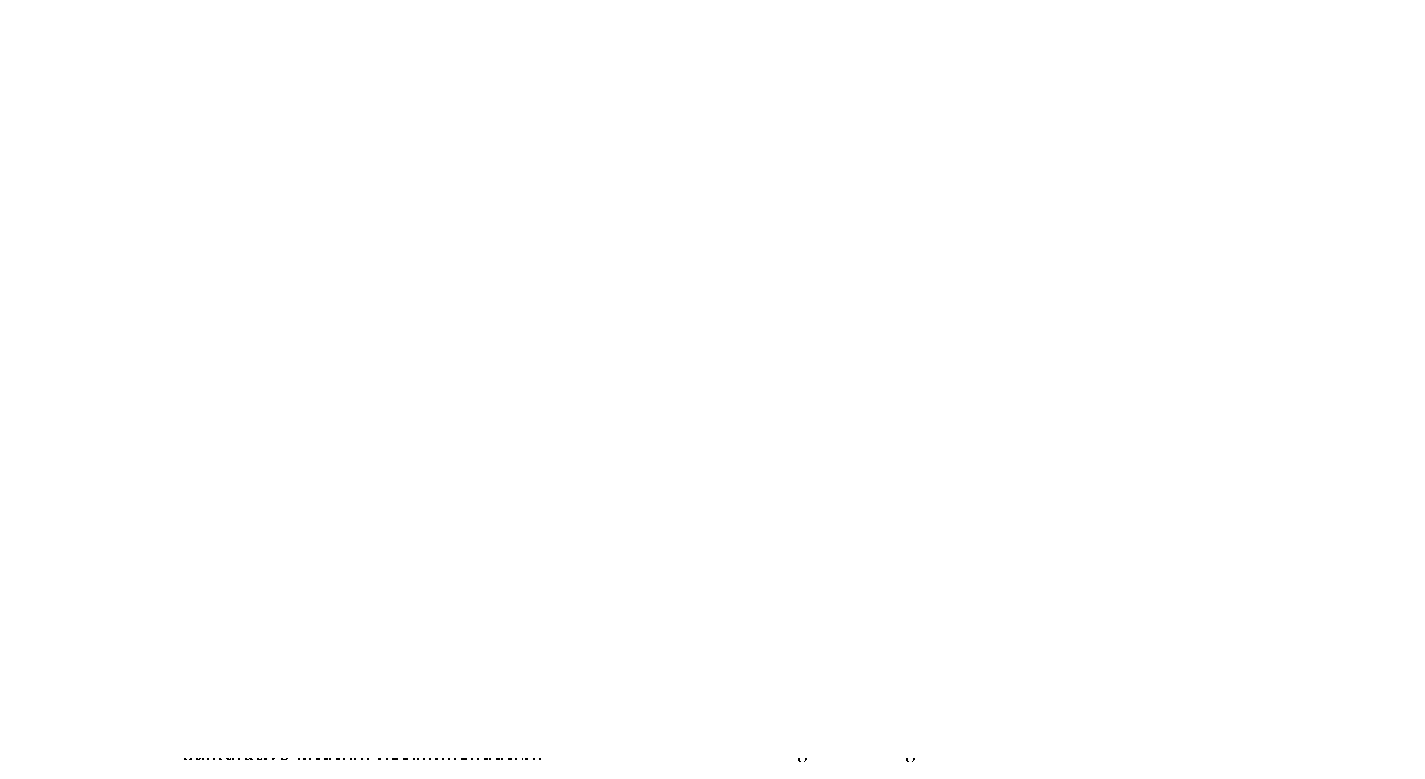
\includegraphics[width=4.5in]{./images/system.eps}
%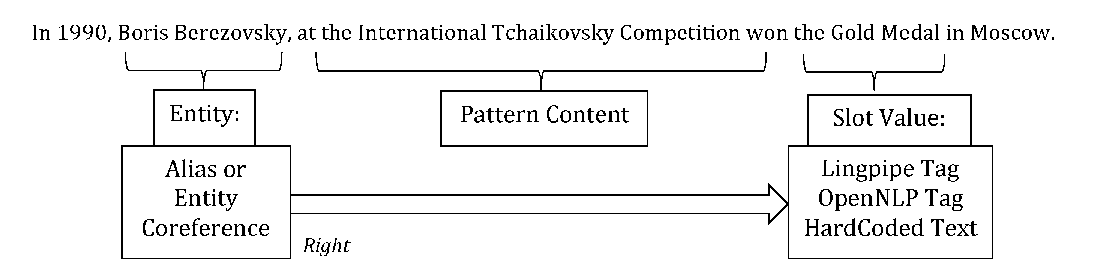
\includegraphics[width=6in]{./images/Pattern.eps}
%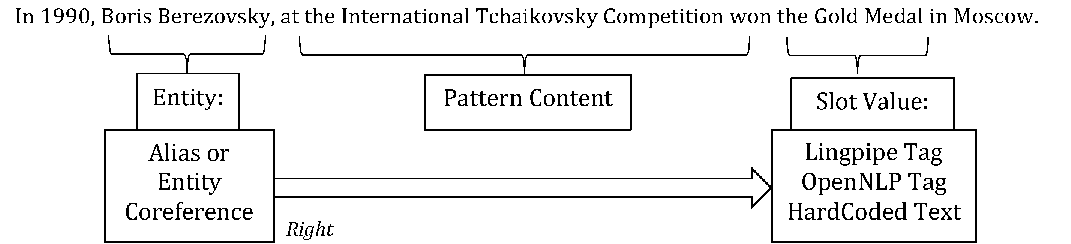
\includegraphics[width=6in]{./images/Pattern-eps-converted-to.pdf}
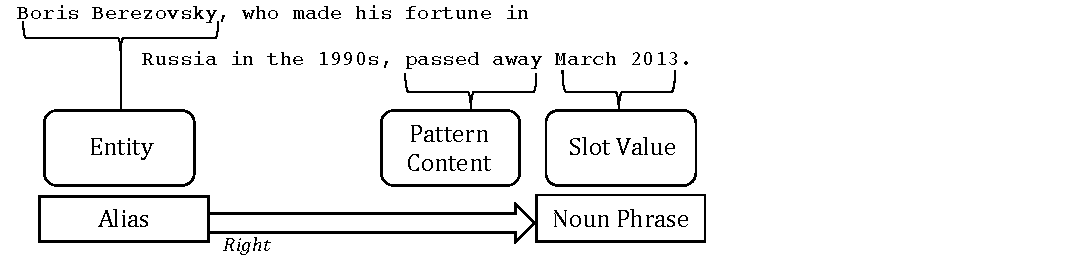
\includegraphics[width = 11cm]{./images/Pattern-crop.pdf}
% cropped pdf created using $ pdfcrop Pattern.pdf
%\vspace*{-.1in}
\caption{Pattern matching for rule evaluation. The slot value is on the right side of the 
entity. The pattern context discovered is `passed away' with a value of `March 2013'. This conforms to type II of our pattern categories.}\label{fig:pattern}
%\vspace*{-.2in}
\end{figure}
 
\textbf{Type I.} This pattern type is driven by the entity type.
For example, in pattern $\langle$\texttt{PER, FounderOf, \textit{founder}, right, ORG}$\rangle$ the \texttt{PER} 
tag means the entity we are finding slot values for is a PER entity;
\texttt{FounderOf} means this is a pattern for FounderOf slot.
\textit{founder} is the word we match in a sentence - the content of pattern occuring in the sentence;
\texttt{right} means that we are going to the right part of the sentence to match the pattern and find the slot value;
ORG means the slot value should be a ORG entity to the right of the entity.

\textbf{Type II.} This pattern type, after finding a matching pattern content, looks for a noun phrase (NP)
that is representative of the slot value.
For example, pattern $\langle$\texttt{PER, AwardsWon, \textit{awarded}, right, NP}$\rangle$
is looking for a noun phrase after the \textit{awarded} that may represent an award.
Titles and awards are not named entity tagged hence the use of the part of speech tagger to fetch the noun phrases.

\textbf{Type III.} These types of facts are best discovered by hard coding the slot values.
Examples of these include time phrases: $\langle$\texttt{PER, DateOfDeath, \textit{died}, right, \textit{last night}}$\rangle$.
In this pattern, the phrase \textit{last night} is exactly searched in the text {last night} to the right of the term \textit{died}.
The intuition behind this pattern is in news articles that report events in the past relative to the article. 
For example, an article will mention that  
a person died `last night' instead of mentioning precise date-time information.
Additionally, part of speech taggers and name entity extractors did not label these terms such as 
\textit{last night} as a DATE entity. 


\subsection{Constraints and Inference}%\ceg{what specifically about the algorithm causes duplicates and errors? --- I asked Yang to elaborate on this as he is more familiar but still not sure what's causing those issues} 
\label{sec:constraintsandinference}

Our data set contains some duplicate webpages, webpage texts with similar content, 
and some of the entity tags are incomplete.
This causes some duplicates or highly similar content in the extracted list. 
We implement a filter to remove duplicates or the fact extractions that match patterns that are general and highly susceptible to be noisy.
The data contains duplicates and incorrect extractions.
We define rules to read ordered sets of facts to sanitize the output.
The input is processed in time order, in a tuple-at-a-time fashion to allow rules to discover noisy slots 
that appears in close proximity.
%We found that the proximity of an extraction has a high correlation on the presence of duplicates. 
We define two classes of rules: \textit{deduplication} and \textit{inference} rules.

The output contains many duplicate entries.
As we read the list of extracted slots we create rules to define ``duplicate''.
Duplicates can be present in a window of rows; we use a window size of 2 meaning we only be adjacent rows.
Two rows are duplicates if they have the same exact extraction or if the rows have the same slot name and a similar slot value or if the extracted sentence for a particular slot types come from the same sentence.

New slots can be deduced from existing slots by defining inference rules.
For example, two slots for the task are ``FounderOf'' and ``FoundedBy''.
A safe assumption is these slot names are biconditional logical connectives with the entities and slot values.
Therefore, we can express a rule ``$X$ FounderOf $Y$'' $\leftrightarrow$ ``$Y$ FoundedBy $X$'' where $X$ and $Y$ are single unique entities.
Additionally, we found that the slot names ``Contact\_Meet\_PlaceTime'' could be inferred as ``Contact\_Meet\_Entity'' if the Entity was a FAC and the extracted sentence contained an additional ORG/FAC tag.
We also remove erroneous slots that have extractions that are thousands of characters in length or tool small.
Errors of extracting long sentences can typically be attributed to poor sentence parsing of web documents.
We have some valid ``small'' extractions. For example, a comma may separate a name and a title (e.g. ``John, Professor at MIT'').
But such extraction rules can be particularly noisy, so we check to see if the extracted values have good entity values.


\section{Evaluation}
\label{sec:results}

We evaluate the effectiveness of extracting slot values for 139 entities.
We look at the baseline coverage for entities and slot names we present in a 500M page snapshot of the English web.
We estimate the precision and recall of our extractions over several extracted fact. 


Our system was developed on a 32-core server described in Table~\ref{table:serverspec}.
Each document is annotated using a name entity extraction and in document coreference.
A bundle of documents are serialized into chunks and encrypted.
The total size of the data after compression and encryption is 4.5TB~\footnote{TREC Knowledge base acceleration stream corpus is available  http://aws-publicdatasets.s3.amazonaws.com/trec/kba/index.html}.
Data is ordered into 11952 date-hour buckets ranged from 2011-10-05-00 (5th of October 2011, 12am)
until 2013-02-13-23 (13th of Feburary 2013, 11pm).
The first four months of data (October 2011 - February 2012) is for training purposes, 
and we use this portion for rule and pattern creation and tuning.
The data set contains text from several web page types as listed in Table~\ref{table:documentsDist}.
%To have a sense of the scale of objects and compression as an example a 6mb gpg.xz files would become 45 mb thrift objects which can contain a couple of thousand StreamItems depending on their size.
%Some of the documents have null values for their annotation fields. The source code of our system is stored as an open source project where enthusiasts can also contribute to \cite{github}, also the relevant discussion mailing list is accessible here \cite{googlegroups}.
 
\begin{table}
\caption{Benchmark Server Specifications}
\centering
\label{table:serverspec}
\begin{tabular}{| c | p{4.8cm} |}
\hline 
\textbf{Spec} & \textbf{Details} \\ \hline
Processor & 32 core AMD Opteron\textsuperscript{TM} 6272 \\ \hline 
OS & CentOS release 6.4 Final \\ \hline 
Software Stack & GCC version 4.4.7, Java 1.7.0\_25, Scala 2.9.2, SBT 0.12.3 \\ \hline 
 RAM & 64GB\\ \hline 
 Drives & 2x2.7TB disks, 6Gbps, 7200RPM\\ \hline 
\end{tabular} 
\end{table}
 
\begin{table}
\caption{Document Chunks Distribution }
\centering
\label{table:documentsDist}

\begin{tabular}{|p{3.8cm}|p{3cm}|}
\hline 
\textbf{Document Type} & \textbf{\# of Documents}\\ 
\hline 
Arxiv & 10988  \\ \hline
 Classified & 34887  \\ \hline
 Forum & 77674  \\ \hline
 Linking & 12947  \\ \hline
 Mainstream News & 141936  \\ \hline
 Memetracker & 4137  \\ \hline
 News & 280629  \\ \hline
 Review & 6347 \\ \hline
 Social & 688848 \\ \hline
 Weblog & 740987  \\ \hline
%\hline 
\end{tabular} 
\end{table}


 
 
 
We develop 172 extraction patterns covering each slot-name/entity-type combinations.
%Our final submission was named \textit{submission\_infer}. 
%Our results are as follows: Document extraction using query entity matching with aliases, sentence extraction using alias matching and co-reference.
%Slot extraction using patterns, NER tags and NP tags.
Out of the 500M documents and 139 entities we found 158,052 documents containing query entities, 17,885 unique extracted slot values for 8 different slots.
We did not get any results from 31 entities missing and 4 slots.

%On the performance of our initial submission run we performed random sampling via two processes, the results of which are according to Table~\ref{table:initialresult}.
In Table~\ref{table:initialresult} we performed two samples of a baseline and estimate the correctness of the extractions.
%\ceg{Add here how the baseline is different from the final submission}
The first was addressing the overall performance measures of the system, e.g.\ precision and recall.
The latter experiment was performed over an enhanced version of the system; we included the aliases from WP API, the alias generation process, and some additional patterns. 
We produced accuracies in range of  54\% and 55\%.
We classify the errors into two sets, an incorrect entities and incorrect extractions.
We found 15\% and 17\% incorrect entity names and we identified 27\% and 30\% incorrect value extracted across all entities and slot types.
The majority of errors were regarding poor slot value extraction patterns and incomplete aliases.

\begin{table}
\caption{Sampled accuracy of the results of the extracted facts.}
\centering
\label{table:initialresult}

\begin{tabular}{| c | c | p{2cm} | p{13mm} |}
\hline 
 & \textbf{Correct} & \textbf{Incorrect Entity name} & \textbf{Incorrect Value} \\ 
\hline 
Sampling \#1 & 55\% & 17\% & 27\% \\ 
\hline Sampling \#2 & 54\% & 15\% & 31\%  \\ 
\hline 
\end{tabular} 
\end{table}


%\ceg{Probably should add again here a reason why our method is different from the baseline.}
After enahncing the system via better and more extraction patterns  we provide more detailed statistics, as displayed in Table~\ref{table:finalresultrecall} and Table~\ref{table:finalresultaccuracy}.
Table~\ref{table:finalresultrecall} shows the recall for each slot name. 
Entities can have different coverages across the entire web, some were more popular (William H. Gates) or less well known such as (Stevens Cooperative School).
Similarly, slot names have various coverages for example \textit{Affiliate} is more probable across the entities when compared to \textit{AwardsWon}. %\ceg{(define `entity coverage' here)}
The slot name \textit{Affiliate} has was extracted the most number of times; \textit{AwardsWon} contained the next fewest with 38 instances found. 
,  affiliations of an organization the following cases have been enumerated \cite{tackbp}: 

An affiliate relationship can be defined in three general ways~\cite{tackbp}:
\begin{itemize}
\item  A relationship consisting solely of the two groups
interacting in a specific event context is not enough evidence to constitute a religious/political affiliation; 
\item Former political or religious affiliations are correct responses for this slot;
\item  Any relation that is not of parent-child form; a sub-organization is not an affiliate its parent organization but rather a Memberof.
\end{itemize}
Affiliate is a generic slot name; extracting affiliate relationships is difficult because the actual relationship must be determined.
Our patterns for this relationship led to noisy results.

However, less ambiguous slot names (AssociateOf) obtained higher accuracy but we have recall.
We developed patterns that explicitly expressed these relationships but we did not create enough patterns to 
express all forms of those slot names.


Table~\ref{table:finalresultaccuracy} addresses the relative accuracy measure per slot value.
\textit{AssociateOf} has the highest accuracy with 63.6\% and \textit{Affiliate}, \textit{Contact\_Meet\_PlaceTime} and \textit{EmployeeOf} have the lowest with lowest of 1\%, 1\% and 5\% accuracy respectively.


\begin{table}[t]
\caption{Recall Measure: Generic slot names like affiliate had the most recall, compared to less popular slot names e.g. DateOfDeath}
\centering
\label{table:finalresultrecall}
\begin{tabular}{|l|p{13mm}|p{22mm}|}
\hline 
 \textbf{Slot Name} & \textbf{Instances Found} & \textbf{Entity \hspace{5 mm} Coverage} \\ 
\hline 
Affiliate & 108598 & 80 \\ \hline 
AssociateOf & 25278 & 106 \\ \hline 
AwardsWon & 38 & 14 \\ \hline 
Contact\_Meet\_Entity & 191 & 8 \\ \hline 
Contact\_Meet\_PlaceTime & 5974 & 109 \\ \hline 
DateOfDeath & 87 & 14 \\ \hline 
EmployeeOf & 75 & 16 \\ \hline 
FoundedBy & 326 & 30 \\ \hline 
FounderOf & 302 &  29 \\ \hline 
Titles & 26823 & 118 \\ \hline 
TopMembers & 314 & 26 \\ \hline 

\end{tabular} 



\caption{Accuracy Measure: Accuracy of AffiliateOf was the best and Affiliate applied poorly due to ambiguity of being an affiliate of somebody/something}
\centering
\label{table:finalresultaccuracy}
\begin{tabular}{|l|p{10mm}|p{10mm}|p{11mm}|}
\hline 
 \textbf{Slot Name}  & \textbf{Correct} & \textbf{Wrong Entity} & {\small \textbf{Incorrect Value}} \\ 
\hline 
Affiliate & 1\% & 95\% & 5\% \\ \hline 
AssociateOf & 63.6\% & 9.1\% & 27.3\%  \\ \hline 
AwardsWon & 10\% & 10\% & 80\%  \\ \hline 
Contact\_Meet\_Entity & 21\% & 42\% & 37\%  \\ \hline 
Contact\_Meet\_PlaceTime & 5\% & 20\% & 85\%  \\ \hline 
DateOfDeath & 29.6\% & 71\% & 25\%  \\ \hline 
EmployeeOf & 5\% & 30\% & 65\%  \\ \hline 
FoundedBy & 62\% & 17\% & 21\%  \\ \hline 
FounderOf & 50\% & 0\% & 50\%  \\ \hline 
Titles & 55\% & 0\% & 45\%  \\ \hline 
TopMembers & 33\% & 17\% & 50\%  \\ \hline 

\end{tabular} 
\end{table}




\section{Discussion}

%In this section we address some of the challenges that we faced during the course of this project. We started 
%off by trying to use the off-the-shelf tools for this task. We started 
%by using Scala/Spark~\cite{ferc11} to benefit from the parallelization 
%performance there. Unfortunately Spark was not performant and the distributed reliability overhead 
%was much more than tolerable. We moved on to use Scala parallelization  framework itself, and unfortunately it did not satisfy our needs as well; there was 
%excessive memory overhead on map-reduce jobs. We migrated the core of the 
%system to Java Parallelism APIs and that was not good enough either, we still demanded 
%better. So we built our own parallel system which in actual performance had 
%the least of overhead, the least memory consumption and the most robust memory 
%model which avoided unpredictable CPU stalls on garbage collections in 
%processing the corpus.

Table~\ref{table:finalresultrecall} shows the distribution of extracted slot names.
The number of extraction between slot names vary greatly.
Some slots naturally have more results than other slots.
For example, DateOfDeath and CauseOfDeath have some of the fewest entities because only a few entities are deceased.
Some patterns use common words as as part of their patterns causing more extractions.
For example, Affiliate looks for common words like  \textit{and} and  \textit{with} as part of the pattern content.
These words are more common than \textit{dead}, \textit{died} or \textit{founded} in other patterns. 

%As part of future work regarding enhancing precision, we can focus on fixing the wrong entities found, remove noisy tags by the Lingpipe or use more accurate NLP taggers such as Stanford NLP (Due to the fact that Stanford NLP is very slow we avoided using it, as due to speed its use was out of question) and finally use better patterns to enahnce results matched by the patterns.
%On the other hand to increase recall we need to find better aliases and go for more resources to discover other ways that an entity might be addressed (e.g.\ twitter id, website, etc), add powerful patterns that can capture more cases of slot values. We would also use entity resolution methods and other advanced methods to improve 
%the accuracy and recall of entity extraction part. 

%For slot extraction, to improve the performance, we need: 1) Using multi-class classifiers instead of pattern matching method to extract slot values in order to increase both recall and accuracy for slots ``Affiliate'', ``AssociateOf'', ``FounderOf'', ``EmployeeOf'', ``FoundedBy'', ``TopMembers'', ``Contact\_Meet\_Entity'' and so on. 2) For special slots, like ``Titles'', ``DateOfDeath'', ``CauseOfDeath'', ``AwardsWon'', using different kind of advanced methods, e.g.\ classifiers, matching methods. 3) Using other NLP tools or using classifiers to overcome the drawbacks of the LingPipe?s inaccurate tags. The first and second tasks are the most important tasks we need to do.

Some of the entities are popular and appear at a greater frequency in the data set.
For example, a `Corn Belt Power Cooperative' Google search results in 86,800 documents, where as `William H. Gates' returns 3,880,000 documents. 
%\ceg{Add an example of someone who is either much larger of smaller.}
We observed that more than half of the entities appear in less than 10 documents in the data set;
%\ceg{Can we add this figure - } 
a large portion have appeared only once. This magnificient change in coverage support the viability of our seach and filter schemes.

%A theory is that we are falling behind because we are using the cleansed (from HTML tags)
%version of the corpus. We believe there has been a reason that TREC has 
%included the actual HTML document as well as the cleansed version. This 
%definitely will convey some information to us. If it was as easy as reading 
%some clean text they wouldn't bother including so much data for teams to be 
%useless. So we guess is that we are missing some information from not using 
%the actual document. And, we are looking for tokens with entity value set 
%which will depend us dramatically on the accuracy of lingpipe, which is a fast 
%algorithm but is not as good as other NLP tools can be e.g. Stanford NLP.

% Note: Here we discuss why the results are the way they are
% Give pros and cons, talk about how the implemented algorithms
% performed in the actual implementation.
% Answer the `why' question about all the trends in the results section.

The system pipeline architecture is an efficient method of processing the stream of data.
Each hour of in the corpus contains and average of 380 MB of compressed data.
It takes and hour for the system to extract facts from 140 hours worth of data fom the KBA corpus.



\section{Conclusion}

In this paper we described an approach to perform fact extraction over one of the largest data sets to date. 
We generate aliases for Wikipedia entities using an API and extract some aliases from Wikipedia pages text itself.
We process documents that mention entities for slot value extraction.
Slot values are determined using pattern matching over tagged entities in sentences.
Finally post processing will filter, cleanup and infers some new slot values to enhance recall and accuracy. 

We sampled documents from the training data period to generate an initial set of patterns and then use these patterns to generate results.
After manually examining the results, we prune patterns with poor performance and add patterns that may add to extraction coverage.
We use several iterations to find the best patterns.
%We found that it is very time consuming to identify quality patterns.

%We noticed that some tools that claim to be performant for using the hardware capabilities at hand sometimes don't really work as claimed and you should not always rely on one without a thorough A/B testing of performance which we ended up in generating our in-house system for processing the corpus and passing through the filter. Furthermore, on extracting slot values, pattern matching might not be the best options but definitely can produce some good results at hand. We have plans on generating classifiers for slot value extraction purposes. Entity resolution on the other hand was a topic we spent sometime on but could not get to stable grounds for it. Entity resolution will distinguish between entities of the same name but different contexts. Further improvements on this component of the system are required. 


We look to continue exploration of streaming extraction models over this large data set.
Our models are simple and provide a great baseline framework to develop and compare innovative techniques.



% Note: Give a summary of our efforts and the
% high level contribution to society.

% Talk about the things we wanted to do and
% didnt get to do.



\section*{Acknowledgements}
We would like to thank John Frank and NIST for providing the data set.
Christan Grant is funded by a National Science Foundation Graduate Research Fellowship under Grant No. DGE-0802270.






\bibliographystyle{aaai}  

\bibliography{citation}








\end{document}
